%----------------------------------------------------------------------------------------------------------------------------------------------------------%
\chapter{Experimental design}
%----------------------------------------------------------------------------------------------------------------------------------------------------------%
\epigraph{It is common sense to take a method and try it; if it fails, admit it frankly and try another. But above all, try something.}{\textit{Anthony Burgess}}
%----------------------------------------------------------------------------------------------------------------------------------------------------------%
\paragraph{}This Extended Essay has the objective of studying bibliographically the effects of \emph{Staphylococcus aureus} on the human body, as well as the ways humanity has developed to defeat it. Experimentally, it has one main objective, and several secondary ones: answering the research questions posed in the most reliable way I can achieve. Secondarily, I want to improve my lab etiquette and fluidity, protocol-making, how I follow protocols in the lab and how I deal with problems that may arise from them, my staining and microscope use,  and how I work with limited resources.\newline 
The research question I will follow is 
\begin{center}"\emph{What is the prevalence of \emph{Staphylococcus aureus} in our school}?"\end{center}
To which my hypothesis is:
\begin{center}\emph{``About 30\%``}\end{center} 
This hypothesis stems from results I found in a paper published in \emph{The Journal of Infectious Diseases}\cite{kuehnertPrevalenceStaphylococcusAureus2006}. I would also like to know the answer to the question
\begin{center}"\emph{Is the prevalence of \emph{Staphylococcus aureus} affected by gender or age?}"\end{center}
to which my hypothesis, based on the knowledge of how bacteria colonise, is 
\begin{center}\emph{``No``}\end{center}
The variable I will study is the presence or not of the bacterium in question on different subjects, and compare it against their characteristics (such as approximate age and gender). I'll keep as control variables the culture medium, the culture temperature and humidity, as well as the sampling conditions (same kind of sterile cotton swabs, same liquid medium to help with sampling -Ringer-, and same procedure).
%----------------------------------------------------------------------------------------------------------------------------------------------------------%
\section{Variables studied}
\paragraph{}This study studied one dependent variable: the prevalence of \emph{Staphylococcus aureus}, comparing it against two different independent variables: the gender of the subject and the age group of the subject. This will allow me to check for a correlation between these tw
%----------------------------------------------------------------------------------------------------------------------------------------------------------%
\section{Bill of materials}
\paragraph{}The materials used, as well as the quantities used, can be found in the following table. On the left, laboratory equipment and, on the right, reagents, staining agents, and consumables (none of the reagents or staining agents were assembled by me, as they were bought already-made)used:
\begin{center}\begin{figure}[H]\centering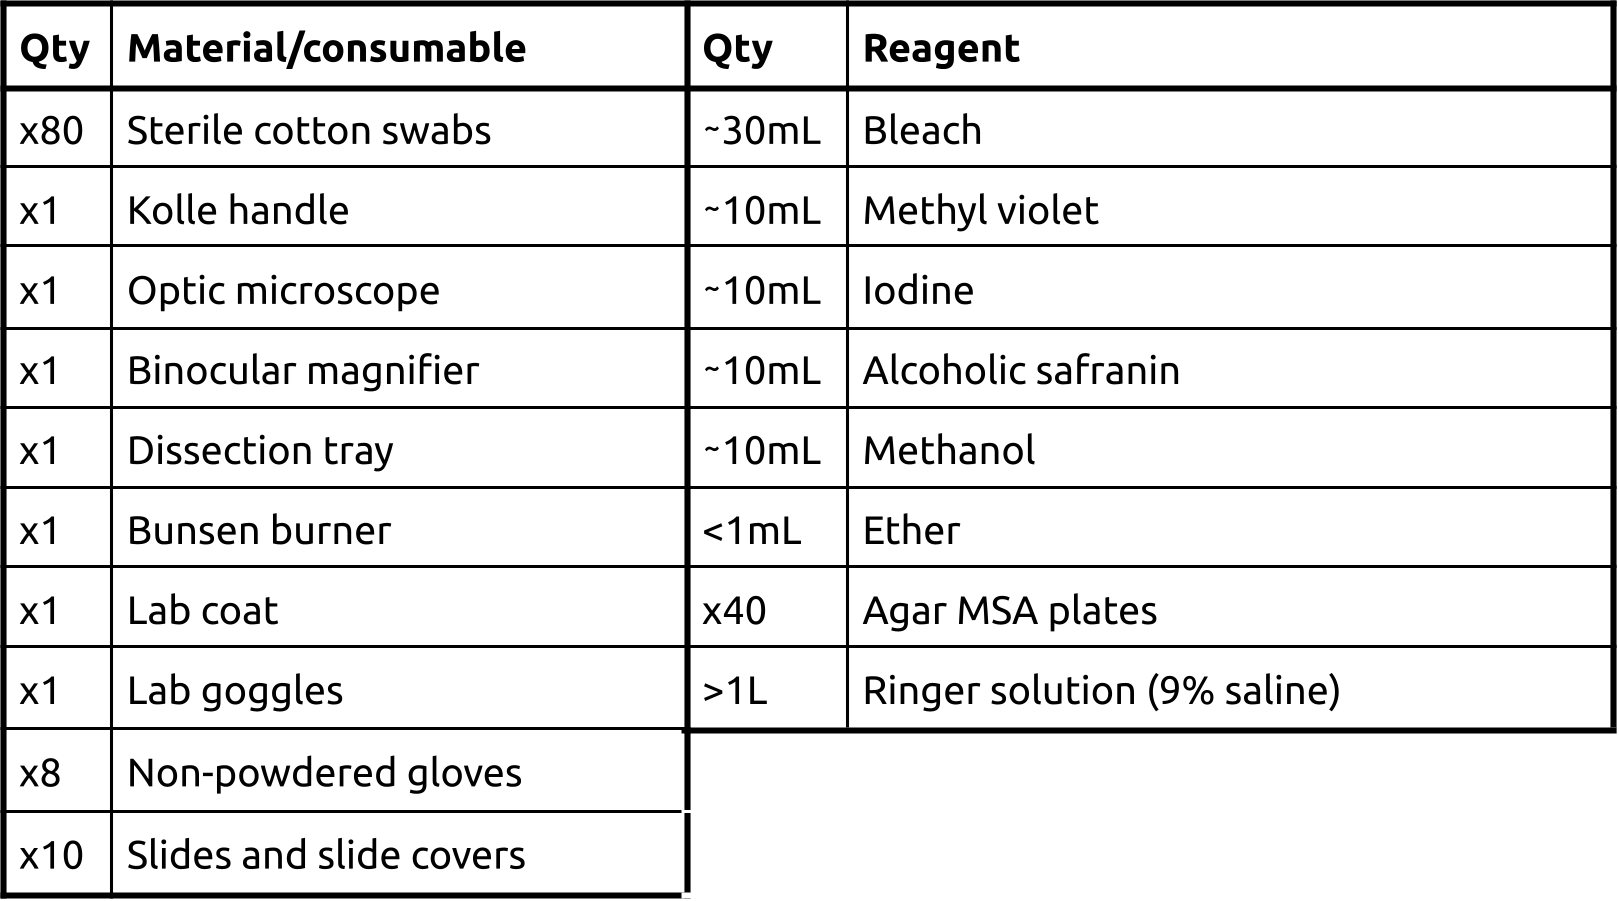
\includegraphics[width=0.90\textwidth]{BOM-1.png}\end{figure}\end{center}
%----------------------------------------------------------------------------------------------------------------------------------------------------------%
\section{Biosecurity and risk mitigation}
\paragraph{}Staph is considered a Biosecurity Level 2 bacterium\cite{cheungPathogenicityVirulenceStaphylococcus2021}. This means that it is associated with a human disease that can pose a moderate human health hazard. In a laboratory where such individua are handled, normal lab etiquette should be followed, as well as avoiding splashes or aerosols, adhering biohazard warning signs present on all material used, and proper surfaces and material disinfection via the use of autoclave.\newline
The risks associated with this bacterium were assessed following the 2020 Biosafety Manual published by the WHO, and proper security measures were followed at all times when handling biohazardous material. No incidents occurred during the research\cite{worldhealthorganizationLaboratoryBiosafetyManual2020}.
%----------------------------------------------------------------------------------------------------------------------------------------------------------%
\section{Protocol followed}
\paragraph{}The protocol followed was designed based on a similar protocol used in many university laboratories\cite{olearyPracticalHandbookMicrobiology1989}, modified to fit the needs of this research paper. This protocol underwent 10 different revisions. It dictates the following steps: \newline\begin{wrapfigure}{r}{0.4\textwidth}\begin{center}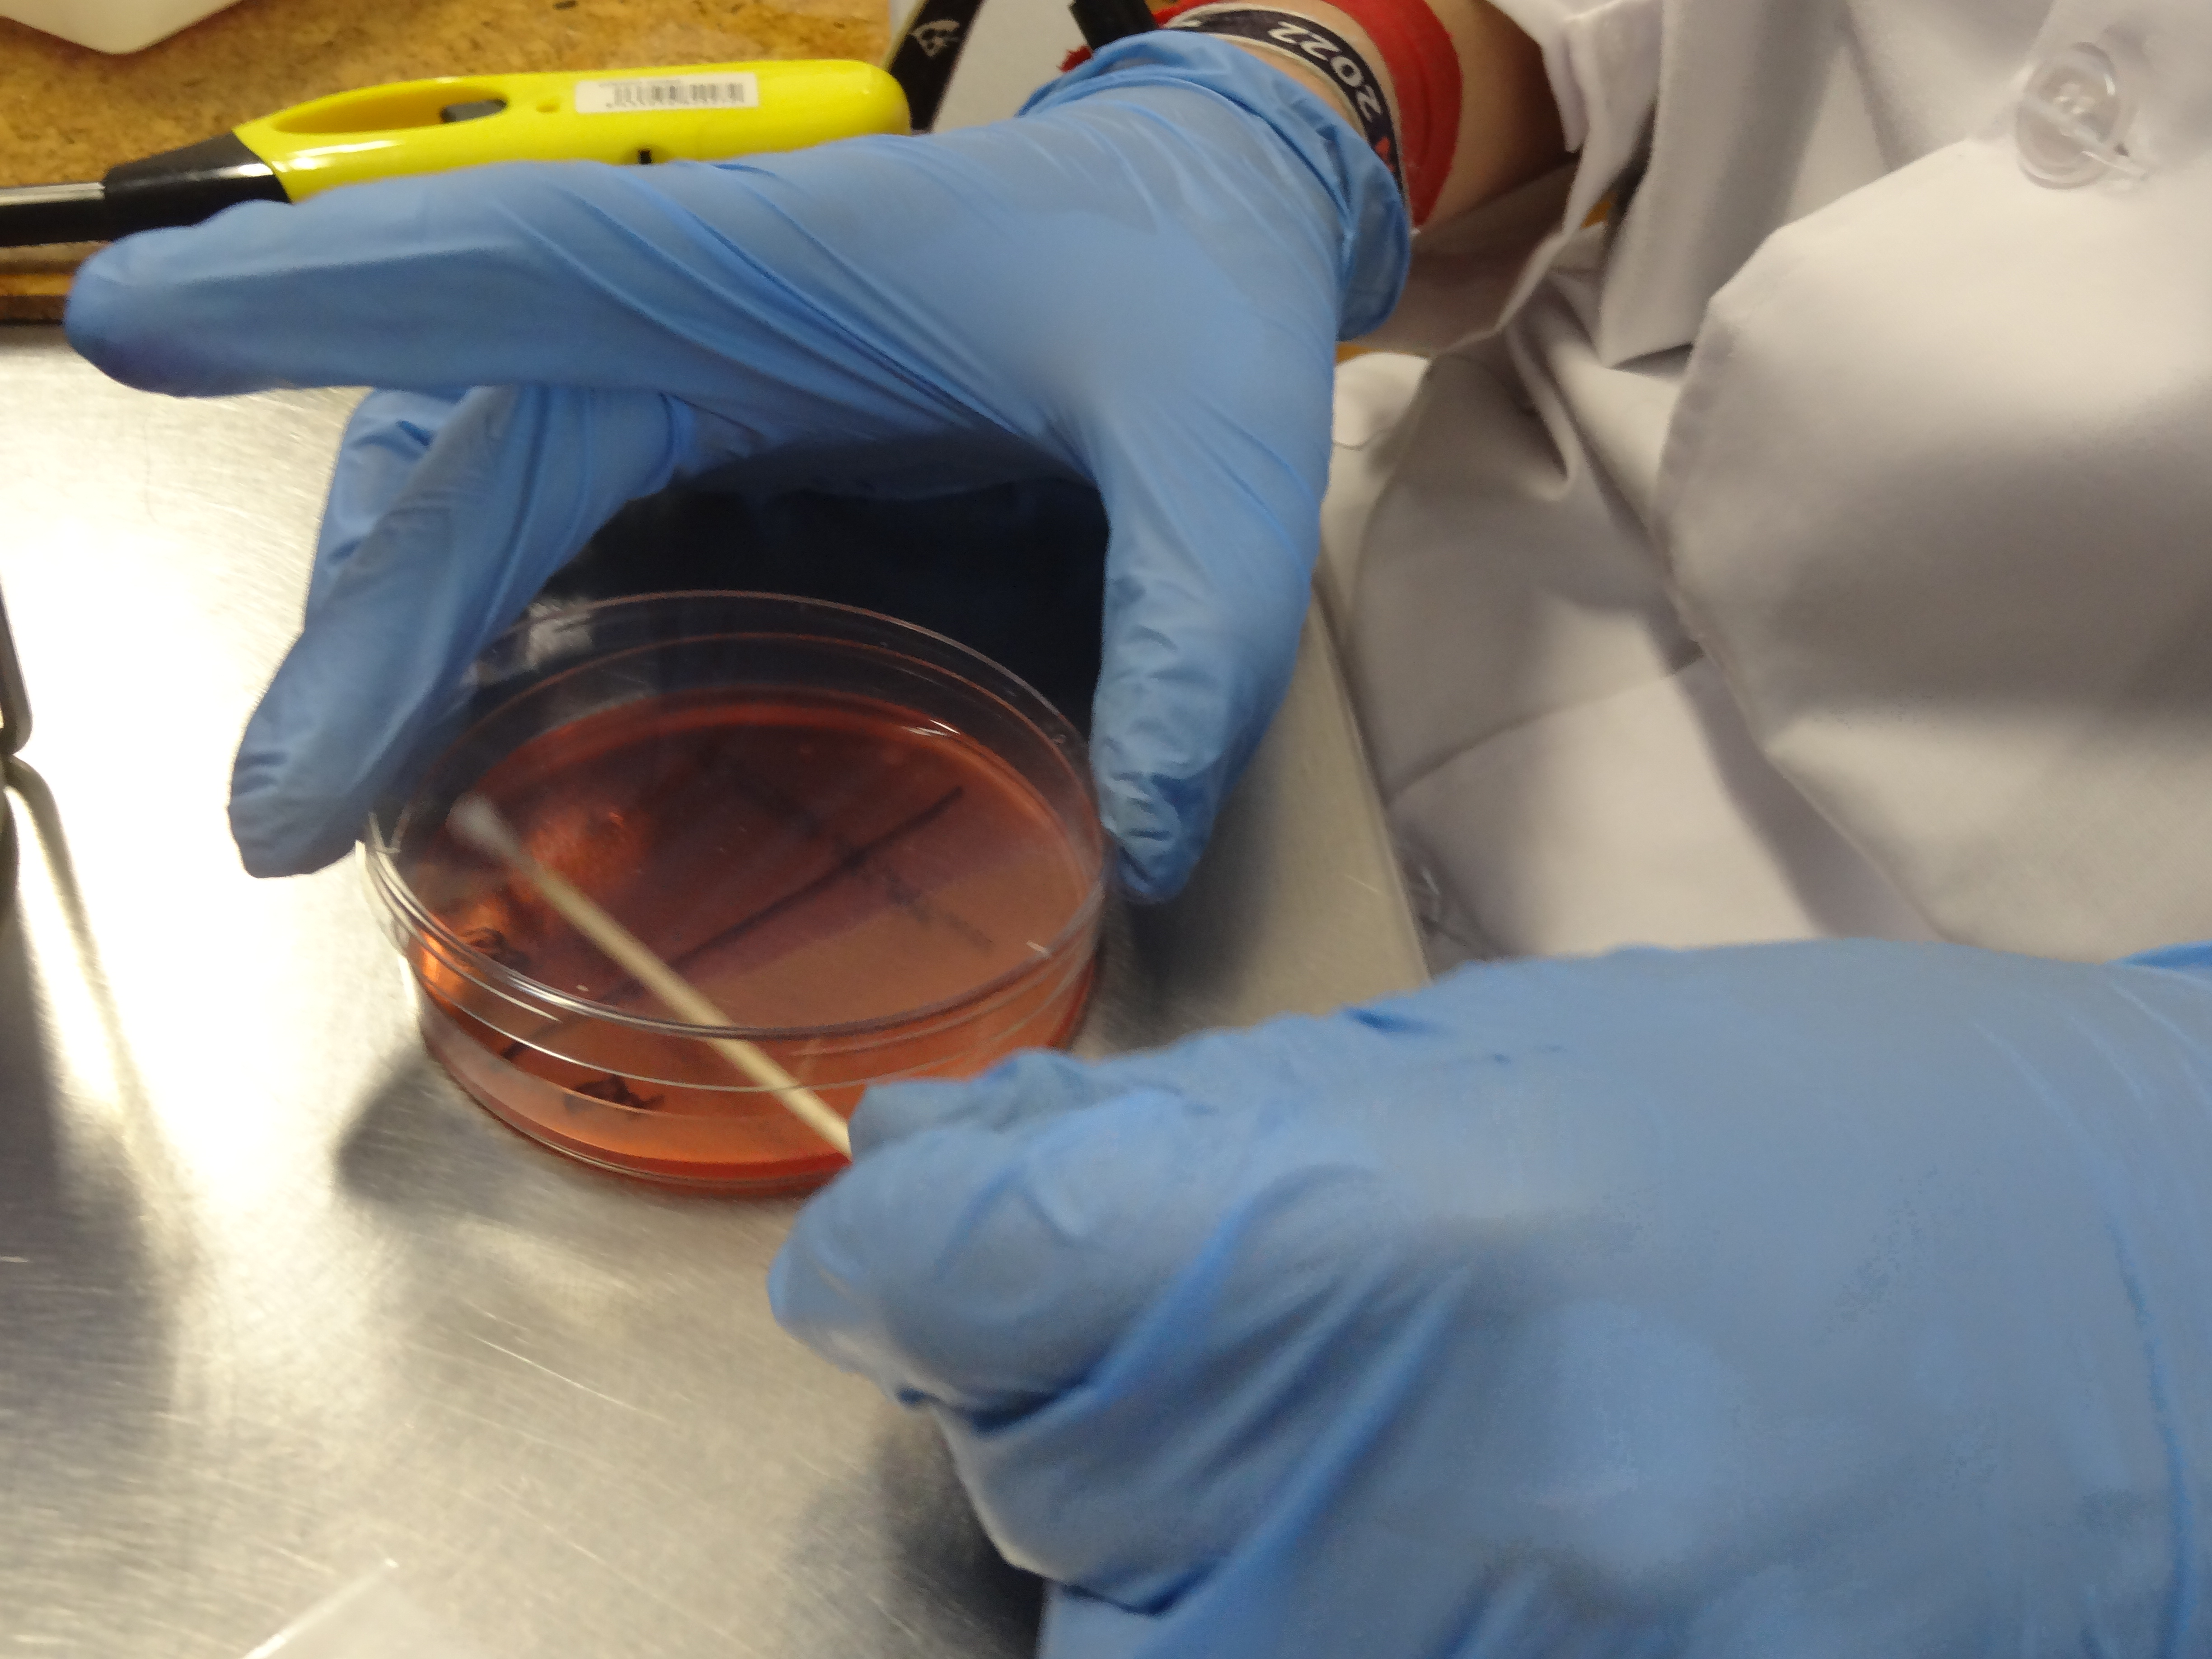
\includegraphics[width=0.38\textwidth]{sampling.JPG}\end{center}\caption{  }\end{wrapfigure}
\begin{enumerate}[label=\arabic*)]
\item Set up the work area; the Bunsen burner should be turned on in such a way that it can cover an acceptable surface to work. Turn it on and try not to break the sterile field.
\item Prepare for the experimentation: wash your hands and put on proper PPE (mask and gloves). Wash your hands again.
\item Divide each Petri dish in 2 parts. Get the subject to wash their hands and observe how they do it. If they don't clean them well enough, teach them proper hand washing techniques.
\item Note down their information, open a sterile swab pack, dip one of the swabs in Ringer solution and swab under their nails or nose. Then, populate the dish with this sample in a zig-zag pattern for one of the halves of the dish.
\item Incubate for 32-48h and observe the results.
\item GRAM stain a sample of the plate and observe it under a microscope.
\end{enumerate}
\begin{figure}[h!] \centering \begin{subfigure}[b]{0.4\linewidth} 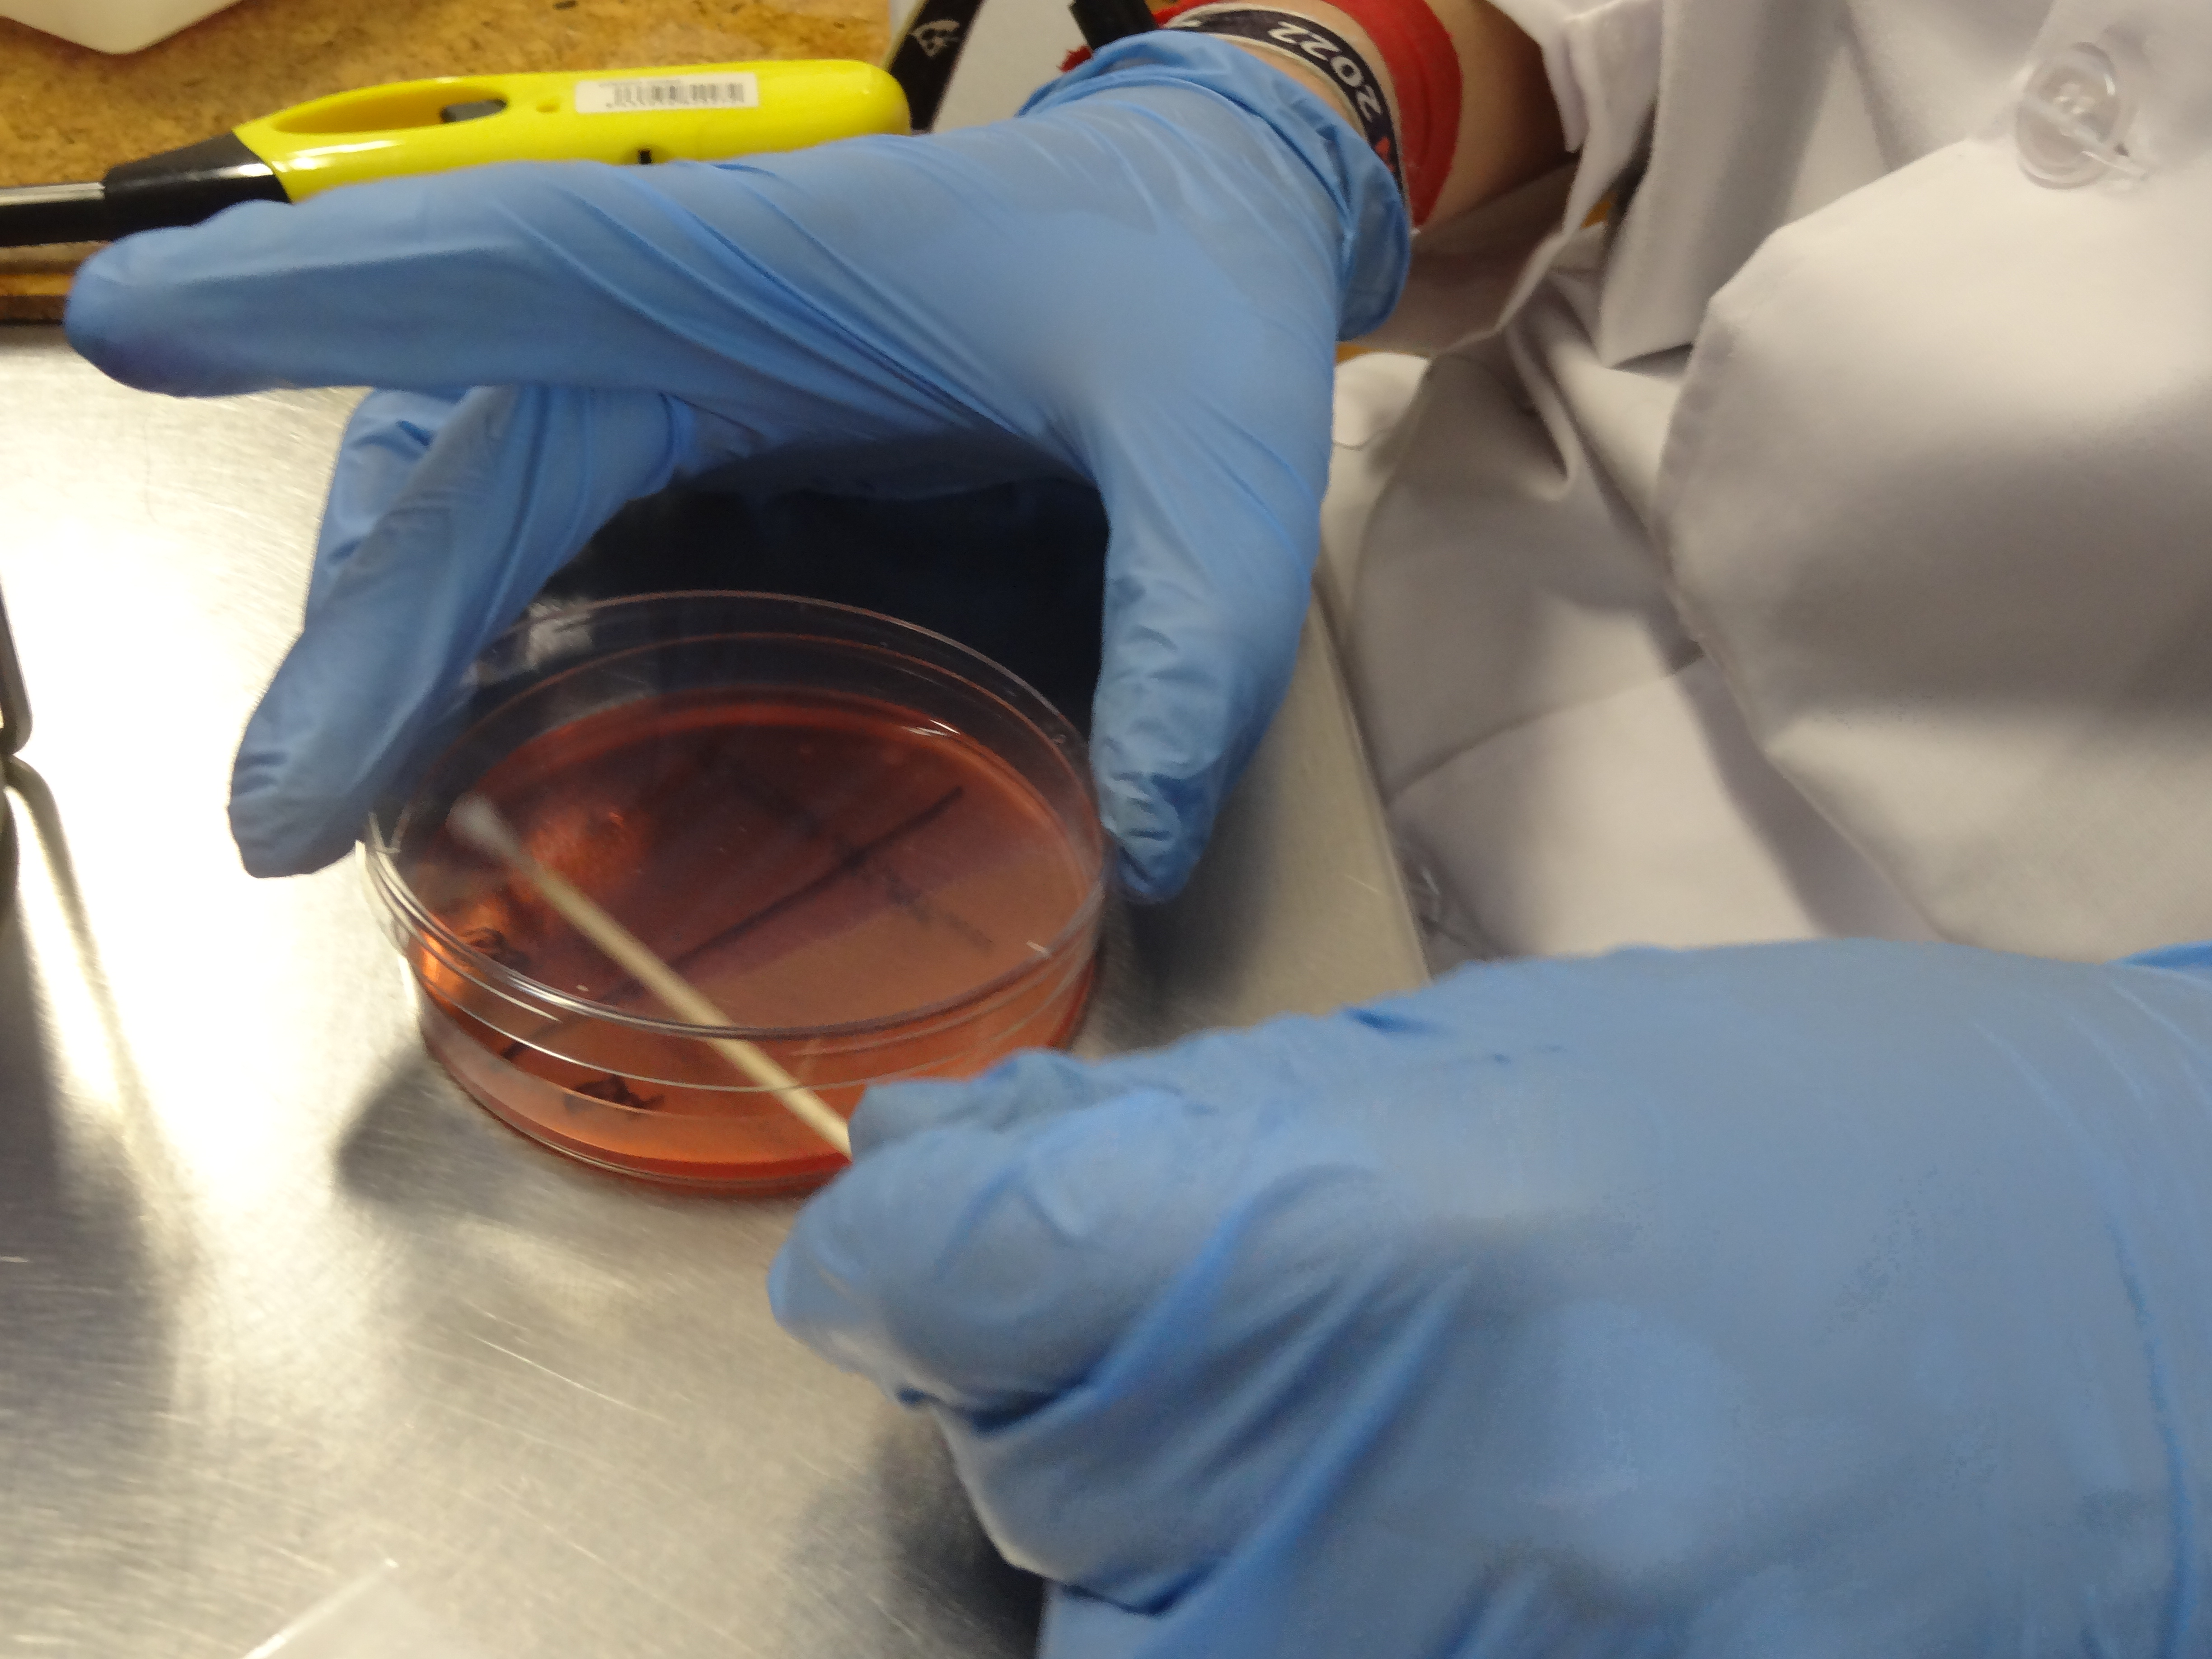
\includegraphics[width=\linewidth]{sampling.JPG} \caption{Photograph of me populating a Petri dish. Source: own} \end{subfigure} \begin{subfigure}[b]{0.4\linewidth} 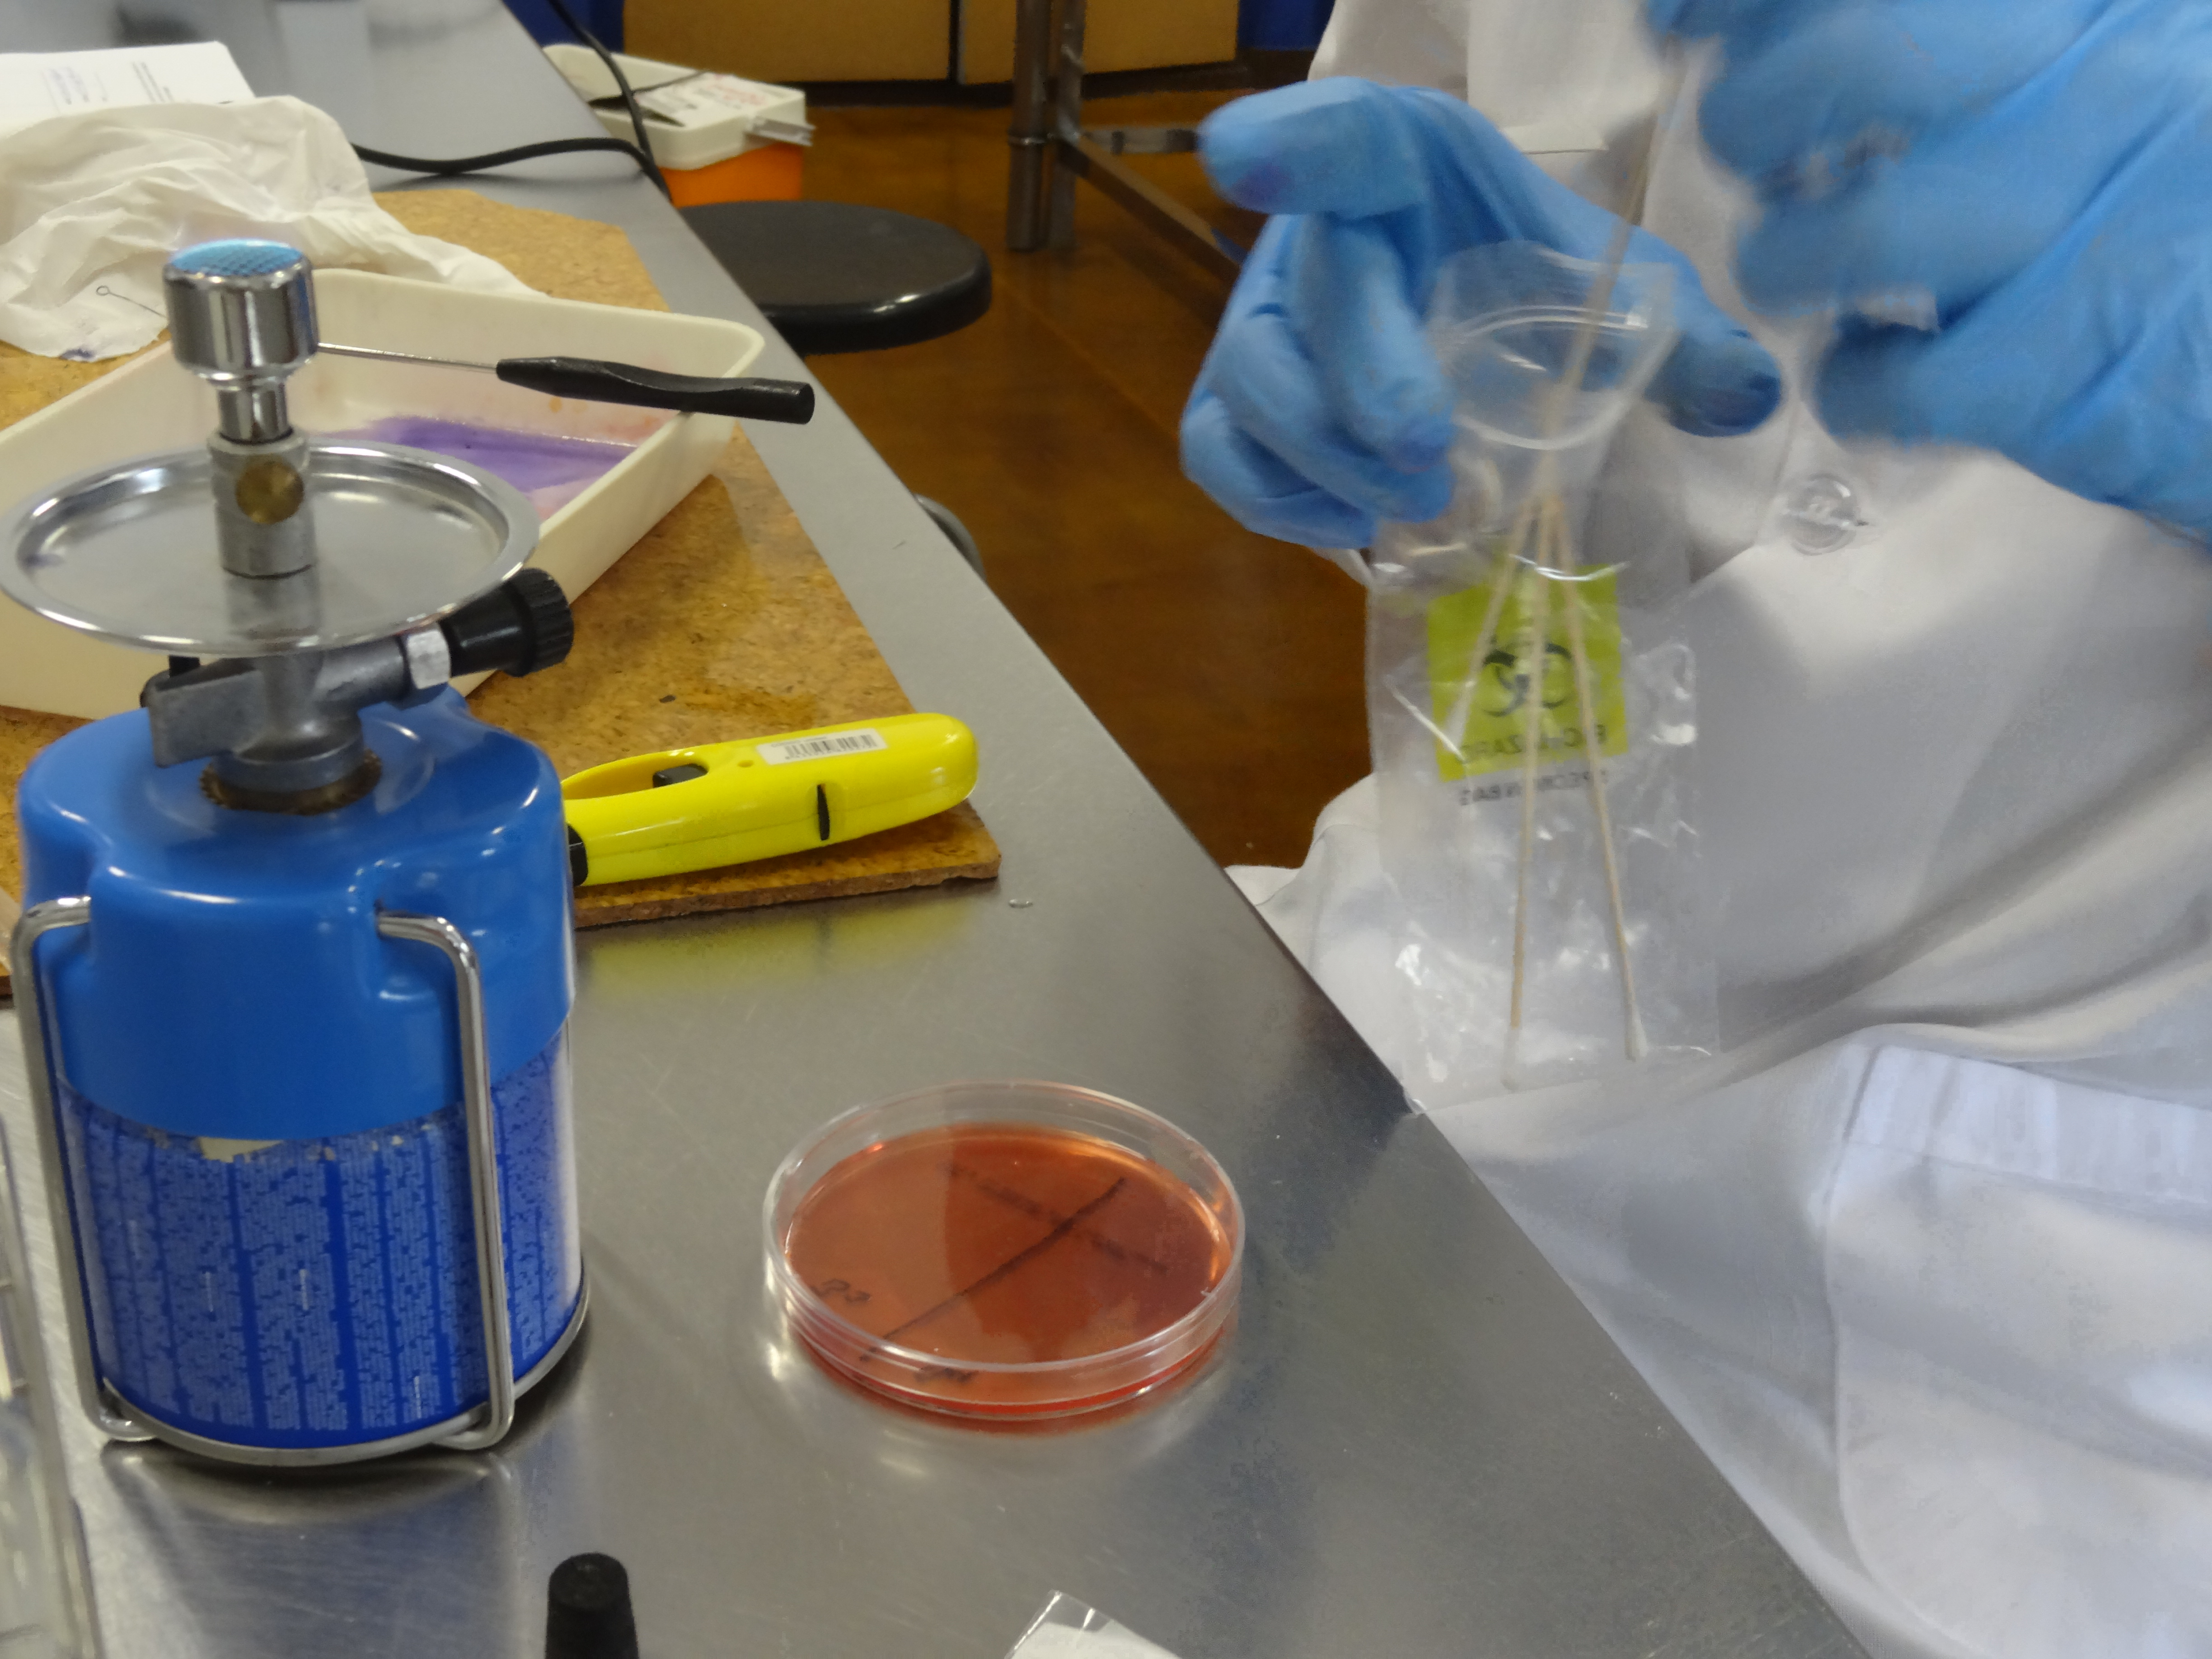
\includegraphics[width=\linewidth]{disposing.JPG} \caption{Photograph of me disposing of contaminated material in a biohazardous materials bag. Source: own} \end{subfigure}\label{fig:coffee}\end{figure}
\newpage